% Report
\documentclass{article}

% Here set the various packages
% Packages to load
\usepackage[english]{babel}
% %%% Support some german text
% \usepackage{ngerman}
% \usepackage[latin1]{inputenc}   % für Umlaute
%%%
% \usepackage[utf8]{inputenc}
\usepackage[T1]{fontenc}
\usepackage{microtype}

%%%
% \usepackage[inline]{enumitem} % Required for the "description" list.

%%% Fix for not hyperlinking citations
\makeatletter
\let\NAT@parse\undefined
\makeatother
\usepackage{hyperref}
% 
\usepackage{cite}
% \ifx\pdfoutput\undefined
% 	\usepackage{graphicx}
% \else
% 	\usepackage[pdftex]{graphicx}
% \fi
\usepackage{graphicx}
\graphicspath{{Figures/}}
\usepackage{amsmath}
% \interdisplaylinepenalty=2500

% Shading of questions. Use the "shaded" environment or the "\hl{}" command.
\usepackage{framed}
% \usepackage[dvipsnames]{color}
\usepackage[svgnames]{xcolor}
\usepackage{soul}
% Nice colours: Gainsboro, LightGoldenrod, LightSteelBlue
% furter ref: https://www.latextemplates.com/svgnames-colors
\definecolor{shadecolor}{named}{Gainsboro}
\sethlcolor{Gainsboro}

%%% Todo margin notes (enable/disable)
\usepackage{todonotes}
% \usepackage[disable]{todonotes}
%%%

%eof

%%%

\title{Programming of Supercomputers\\Worksheet 2}
\author{
	\begin{tabular}{rl}
		Oleksandr Voloshyn& \texttt{<o.voloshyn@tum.de>}\\ 
		Qunsheng Huang& \texttt{<keefe.huang@tum.de>}\\ 
		Tommaso Bianucci& \texttt{<bianucci@in.tum.de>}
	\end{tabular}
}
\date{\today}

\begin{document}

\maketitle
\renewcommand{\abstractname}{Group members's contributions}
\begin{abstract}
	\begin{center}
		\begin{tabular}{rl}
		% Here write the contributions of the members of the group
		Oleksandr Voloshyn:& worked on Task 2 to 5. \\
		Qunsheng Huang:& worked on Task 2 to 5.\\
		Tommaso Bianucci:& worked on Task 1 and Task 6.\\
		\end{tabular}
	\end{center}
\end{abstract}

\section{Task 1: Understanding Parallel Programming Challenges}
\subsection{Concepts description}
\begin{description}
	\item[Race condition]

	It is a concurrent access to data by two different threads in which the outcome of the program changes depending on the order of the accesses. This leads to non-deterministic behaviour of the program.

	\item[Deadlock]

	A condition in which two or more threads are waiting on each other before continuing execution, therefore blocking each other execution indefinitely.
	
	\item[Heisenbug] 

	A bug which occurrence is influenced by the presence of a debugger\todo{TO BE CONFIRMED}, therefore it does not happen during debugging, making it more difficult to solve.
	
	\item[Cache coherency and false sharing] 

	Two processors, each having its own cache, load the same data from memory to their caches. Then processor 1 changes this data in its own cache. \emph{Cache coherency} mechanisms ensure that this change is propagated also to the cache of processor 2, to avoid it to work on old data which is not valid anymore. \emph{False sharing} is an unwanted side effect of cache coherency mechanisms and occurs when two processors load the same cache line but work on different data within this cache line. Each write operation from one processor will cause the other one to have to reload its cache, even if the change was in data which will not be used by the other processor.\todo{Write this in a better form}
	
	\item[Load imbalance] 

	A load imbalance is a situation in which two processors are given different amount of work to perform concurrently. This is usually a cause of performance degradation, as the less loaded processor will have to idle while waiting for the more loaded one to finish.
	
	\item[Amdahl's law] 

	If a program has a fraction $f$ which is parallelizable and and the remaining $(1-f)$ which is inherently sequential, we can estimate the time it takes to execute it on $N$ processors as:
	\begin{align}
		T(N) =& f \cdot \frac{T(1)}{N} + (1 - f) \cdot T(1)\\
		=& T(1) \cdot (1 - f + \frac{f}{N})
	\end{align}
	Therefore $lim_{N\to\infty} T(N) = T(1) \cdot (1 - f)$. So we can see that performance improvement is limited by the non-parallelizable fraction of the program.

	\item[Parallelization overhead] This is the additional performance cost caused by managing the parallelization, as e.g. the additional time spent in communication, synchronization, creating the new threads.
	
	\item[Floating-point arithmetic challenges] ~\todo{Review this}
				\begin{description}
			\item[Comparisons] Comparing floating point numbers can be challanging because due to errors and rounding they could be slightly different. Also, finite precision representation does not allow for all values to be represented, therefore it is not possible to precisely compare with any arbitrary value.

			Checking \verb!a == b! is therefore dangerous, while an acceptance range should be used, i.e. \verb!fabs(a-b) < tolerance!.
			\item[Definition of zero and signed zero] The IEEE 754 standard allows for both $+0$ and $-0$ representation: their exponent and mantissa is $0$ for both, but the sign bit can be 0 ($+$ case) or 1 ($-$ case).
			\item[Cancellation or loss of significance] Cancellation is an undesired side effect coming from performing subtractions in finite precision floating point arithmetics: if we subtract two values which are similar in magnitude, we obtain a result which is very small in magnitude but with increased relative error compared to the initial values, therefore having less significant digits.
			\item[Amplification and error propagation] Any floating point value given as input to an algorithm is associated with a certain relative error or number of significant digits. The foating point operations which take place in the algorithm may amplify or reduce the relative error on these values, therefore causing the final result to potentially have a very different number of significant digits than the input values. Algorithms which amplify input relative errors are called \emph{unstable}, while those which reduce the relative errors are called \emph{stable}.
		\end{description}
\end{description}

\subsection{Questions}
\begin{enumerate}
	\item \hl{Which of the concepts affect performance but not correctness?}

	False sharing, load imbalance, Amdahl's law and parallelization overhead.

	\item \hl{Which of the concepts affect the correctness of the application?}

	Deadlocks, race conditions, heisenbugs and the floating-point arithmetic challenges.

	Cache coherency is usually an hardware-provided feature: assuming it is correctly implemented it should be just considered as a performance problem. However if the programmer must in some way ensure cache coherency, then there is a risk for correctness issues.

	\begin{enumerate}[label=\Alph*]
		\item \hl{Of these, which are exclusive to parallel programming?}

		Deadlocks and race conditions.

		\item \hl{Of these, which are not exclusive to parallel programming?}

		Heisenbugs and floating-point arithmetic challenges.

	\end{enumerate}

	\item \hl{Which of them can occur in OpenMP applications?}

	All of them.
	
	\item \hl{Which of them can occur in MPI applications?}

	All of them, except for false sharing and cache coherency.
	
	\item \hl{Is cache coherency necessary on MPI applications with a single process and a single thread per rank? Explain.}

	No, if there is no degree of shared memory parallelization there is no need to ensure coherency, as just one thread can touch its memory region.
	
	\item \hl{Is Amdahl's law applicable to strong scaling applications? Explain.}

	Yes, it is precisely designed to model and explain the challanges of strong scaling as it assumes a fixed problem size and an increase in the number of processors.
	
	\item \hl{Is Amdahl's law applicable to weak scaling applications? Explain.}

	No, as explained in the previous answer, Amdahl's law assumes a fixed fraction of the application cost is parallelizable. However by changing the problem size, the parallelizable and inherently sequential fractions may change.

	A law addressing weak scaling is \emph{Gustafson's law}.
	
	\item \hl{Which of these limit the scalability of applications?}

	Amdahl's law, parallelization overheads, load imbalance and false sharing.
	
\end{enumerate}

% % Figure example
% \begin{figure}[h!] % h=here, t=top, b=bottom, p=(extra)page, !=force
%  	\begin{center}
%  		
\includegraphics[width=.9\linewidth]{figure.png} % It searches in the Figures/ folder!
%  		\caption{Caption text}
%  		\label{fig:figureLabelName}
%  	\end{center}
% \end{figure}

\section{Task 2: TotalView GUI}

	\begin{enumerate}
	

	\item \hl{Include a brief description of the following aspects of TotalViews GUI in the report:}
	\end{enumerate}
	\begin{itemize}
	\item \hl{Session Manager}
	
	Manages debugging sessions, see Fig.\ref{fig:sess_manager}. 
	Displays previously configured debugging systems---allowing editing, copying and deleting of preivous settings, and view their respective configuration setups. 
	Available configurations include type of session (parallel/sequential), parallel implementation (poe-linux/MPICH etc.), number of parallel processes, number of nodes, environmental variables and input to parallel program upon startup.
	\begin{figure}[p] % h=here, t=top, b=bottom, p=(extra)page, !=force
		\begin{center}	
		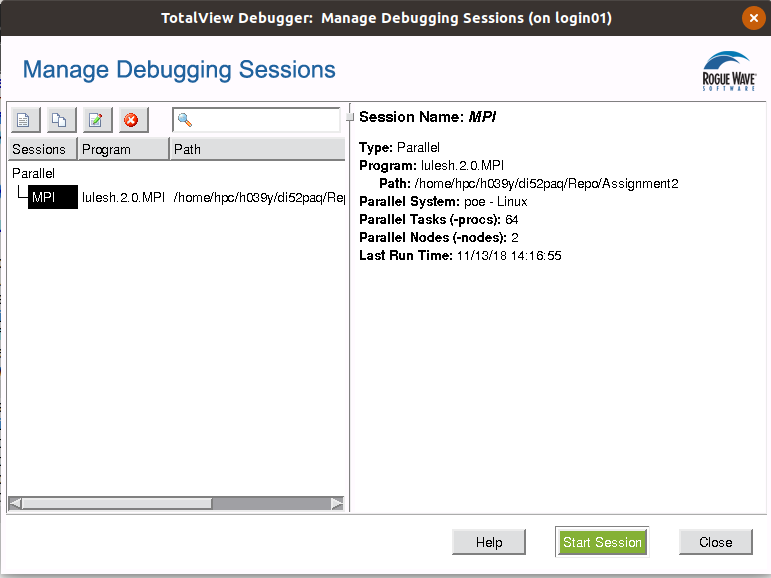
\includegraphics[width=.7\linewidth]{SessionManager.png}
		\caption{Session manager}
		\label{fig:sess_manager}
		\end{center}
	\end{figure}
	\item \hl{Root Window}
	
	Lists all processes and threads controlled by TotalView, see \ref{fig:root_window}. 
	Allows user to "Dive" into processes easily, which launches a process window for the selected process.
	Allows grouping of threads/processes for easier debugging.
	\begin{figure}[p] % h=here, t=top, b=bottom, p=(extra)page, !=force
	\begin{center}
			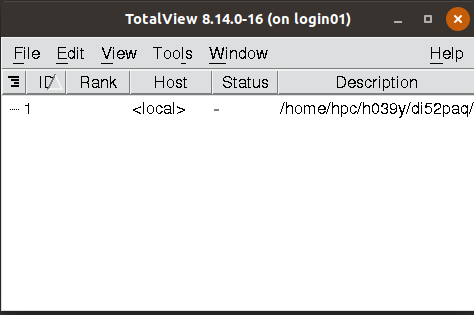
\includegraphics[width=.7\linewidth]{RootWindow.png}
		\caption{Root Window}
		\label{fig:root_window}
	\end{center}
	\end{figure}
	\item \hl{Process Window}
	
	Window for one specific process or thread, see Fig. \ref{fig:proc_window}. 
	Provides information on state of the process and its individual threads. 
	Information provided listed in the various panes below.
	\begin{itemize}
		\item \hl{Stack Trace Pane}
		
		Displays the call stack with any active threads, ie lists the active subroutines of the active thread. 
		Able to move up and down the call stack by clicking on the stack frame (routine name) of interest.
		Stack Frame pane and Source pane updated for the specific routine when it is selected. 
		Local variables are also available in the Local Variables (VAR) Panel.
		\item \hl{Stack Frame Pane}
		
		Displays information on the current thread's variables, ie allows users to see the current/stored values in existing variables. 
		The frame is seen in Fig \ref{fig:diving}.
		\begin{figure}[p] % h=here, t=top, b=bottom, p=(extra)page, !=force
		\begin{center}
			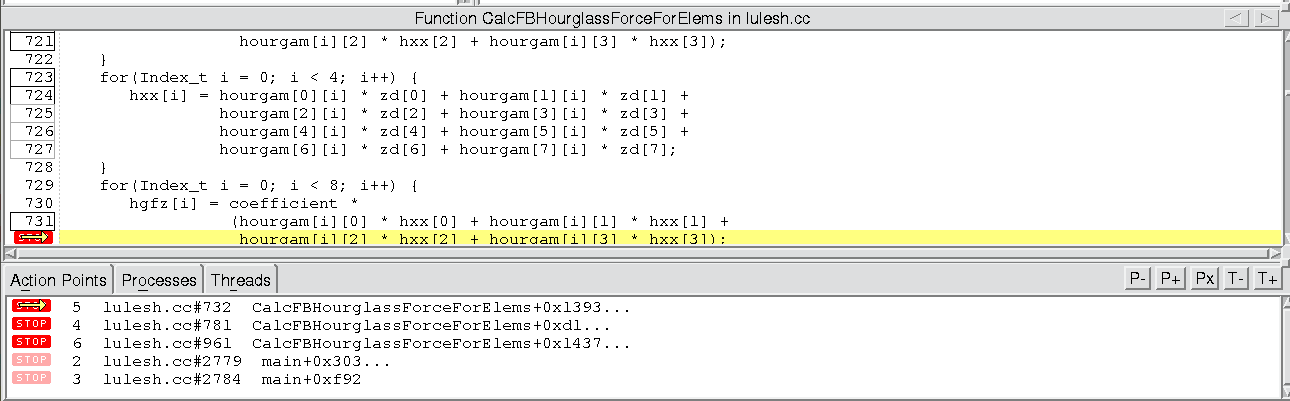
\includegraphics[width=.7\linewidth]{SourceFrame.png}
		\caption{Diving in Function}
		\label{fig:diving}
		\end{center}
	\end{figure}
		\item \hl{Source Pane}
		
		Displays the source code for the main() function of the thread, process or selected routine
		\item \hl{Action Points, Processes, Threads Pane}
		\begin{itemize}
		\item The three tabs can be seen in Fig \ref{fig:action_proc_thread_tabs}.
		\item \hl{Process Tab} 
		
		The processes tab, or Ranks tab for MPI programs, contains a grid. 
		Each block in the grid represents one process. 
		The color of the respective segments indicates the state of the process. 
		\item \hl{Threads Tab} 
		
		The Threads Tab displays information about the state of your threads. 
		Clicking on a thread tells TotalView to shift the focus within the Process Window to that thread.
		\item \hl{Actions Points Tab} 
		
		Action points are specific actions performed when a particular source line is reached. 
		There are four possible actions: breakpoints, barrier points, eval points, and watch points.
		Totalview assigns unique ID numbers for each action point, these are seen in the actions points tab
		\end{itemize}
	\end{itemize}
	\begin{figure}[p] % h=here, t=top, b=bottom, p=(extra)page, !=force
		\begin{center}	
		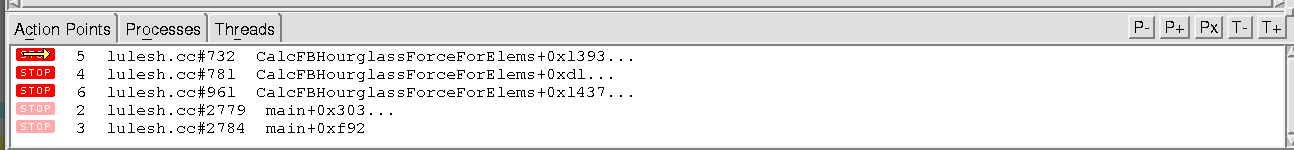
\includegraphics[width=.7\linewidth]{ActionTab.png}
		
		
		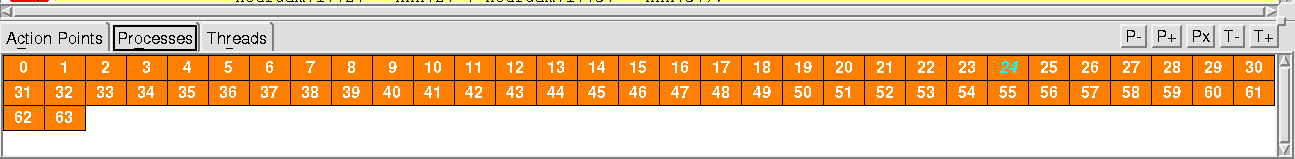
\includegraphics[width=.7\linewidth]{ProcessTab.png}
		
		
		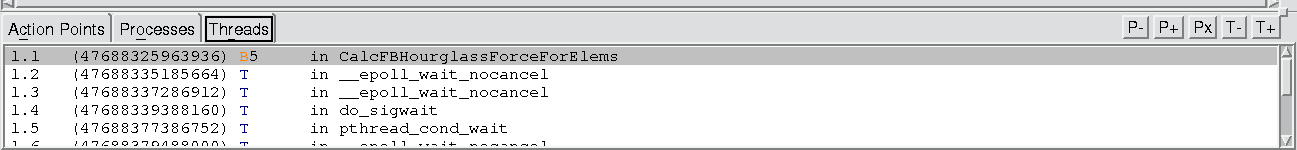
\includegraphics[width=.7\linewidth]{ThreadTab.png}
		\caption{Action, Process \& Thread Tabs}
		\label{fig:action_proc_thread_tabs}
			\end{center}
	\end{figure}


	\begin{figure}[p] % h=here, t=top, b=bottom, p=(extra)page, !=force
		\begin{center}
			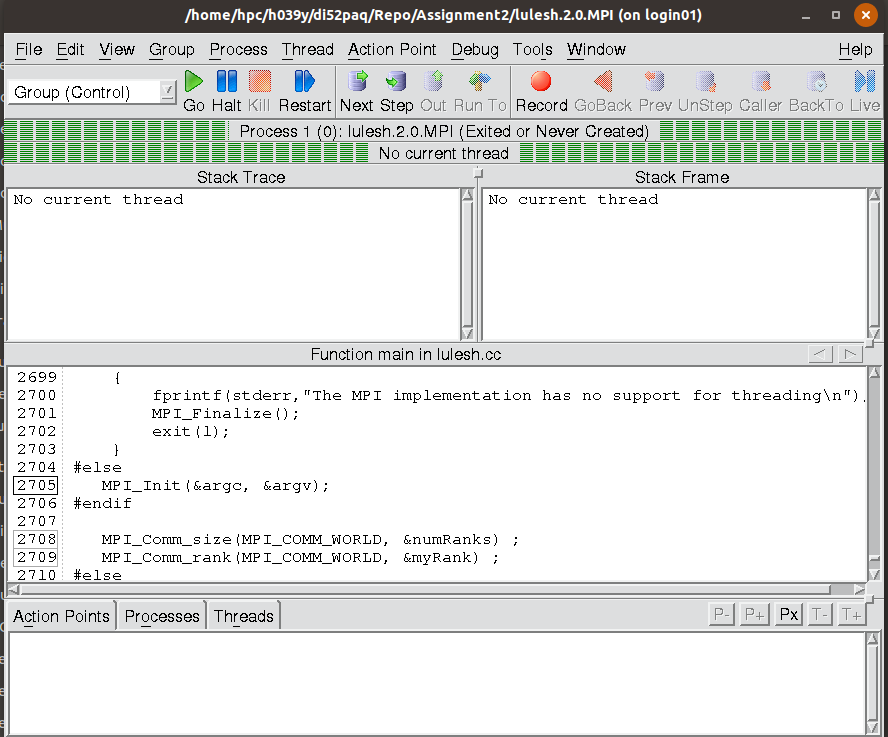
\includegraphics[width=.7\linewidth]{ProcessWindow.png}
		\caption{Process Window}
		\label{fig:proc_window}
		\end{center}
	\end{figure}

	\item \hl{Variable Window}
	
	Displays information about a program's objects. 
	Allows user to change the element values or to cast these values (changing how the value is displayed). 
	You can define fields which change how objects are viewed, for example: expression field (views result of a particular expression, ie. viewing a particular element in an array with expression 'val[3]' instead of 'val'.); type field (changing the data type of the particular element, and so on. 
	The user can also 'dive' into more complex elements to observe or change members of structures or elements of arrays. An example is seen in Fig \ref{fig:variable}.
	
	\begin{figure}[p] % h=here, t=top, b=bottom, p=(extra)page, !=force
		\begin{center}
			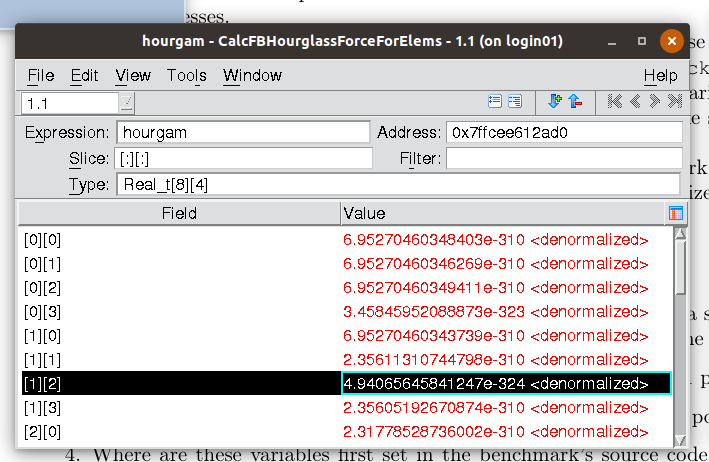
\includegraphics[width=.7\linewidth]{VariableWindow.png}
		\caption{Variable Window}
		\label{fig:variable}
		\end{center}
	\end{figure}
	
\end{itemize}

\section{Task 3: Debugging with TotalView}
\begin{enumerate}
\item \hl{Describe in the report how the above operations are performed in TotalView}
	\begin{itemize}
	\item \hl{Control Execution}
	
	This controls how the user moves through the program. 
	There are a few options available: go, next, step, out, and run to. 
	Go executes the program normally and only stops with the addition of breakpoints. 
	Next runs the one line of code and advances to the next line. 
	Step runs until the next executable statement is reached. 
	Run to allows the user to run normally until a specific selected line. 
	Out is used to execute the return statement and exit a function. 
	All these options are available as clickable buttons along the top of the Process window, seen in Fig \ref{fig:stepping}.
		\begin{figure}[p] % h=here, t=top, b=bottom, p=(extra)page, !=force
		\begin{center}
			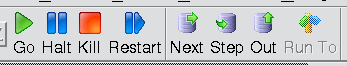
\includegraphics[width=.7\linewidth]{ControlStepping.png}
		\caption{Control Execution}
		\label{fig:stepping}
		\end{center}
	\end{figure}
	\item \hl{Setting breakpoints}
	
	Breakpoints are the simplest form of Action Point availablein TotalView that stop the current threads execution when a specific line is reached. 
	They can be setup prior to running the process by clicking on the specific line number in the Source Pane or right clicking the line number and selecting "Set Breakpoint". 
	The line number will be highlighted and the new breakpoint will be visible in the Action Point tab.
	 Sample breakpoints can be seen in the Action Point tab in Fig \ref{fig:action_proc_thread_tabs}.
	\item \hl{Diving into functions}
	
	"Diving" is the term used by TotalView to focus on a function, process or variable. 
	To dive into a function, one can double-click on the function in the Processes tab or navigate to the function in the source view. 
	An example of diving into a function is seen in Fig \ref{fig:diving}, where we dive into function \verb!CalcFBHourglassForceForElems()!.
	
	\item \hl{View memory (variables and arrays)}
	
	Variables and arrays can be accesed in the Variables window. 
	This is accessed by double-clicking or right clicking and diving into specific variables in the Stack Frame menu. 
	An example is seen in Fig \ref{fig:variable}, where we view the values in array \verb!hourgam! in thread 24.

	\end{itemize}
\item \hl{Give a short explanation on why these operations are important in a debugger.}
	\begin{itemize}
	\item \hl{Control Execution}
	
	Control execution is important when debugging because it allow a systematic manner to execute segments of code. 
	For example, if one needs to pinpoint problematic segments of very large code, perhaps a normal "Run" command with certain breakpoints while observing key variables is a good starting point. 
	On the other hand, if one has a short problematic segment of code, repeatedly running Next to examine the effects of each line of code might be necessary to uncover more insidious bugs. 
	The available options allow for the user to move through code in an extremely flexible manner.
	\item \hl{Setting breakpoints}
		
	Breakpoints are extremely useful when debugging. 
	They cause the program to halt or stop execution at a specific interval for deeper analysis. 
	TotalView also allows for code execution during action points (known as eval points), which is extremely useful for evaluating behavior without having to specifically include calculation of variables of interest inside the examined code. 
	\item \hl{Diving into functions}
	
	Diving into functions allows for increased granularity when running code. 
	If one function is identified to be problematic, having the diving functionality allows the user to also control the execution inside the problematic function---allowing a more fine-grained view of the problematic function.	
	\item \hl{View memory (variables and arrays)}
	
	Most of the time, the side-effect of problematic code is incorrect variables or arrays, ie. data is incorrectly calculated. 
	Viewing specific variables or arrays allows the user to more clearly detect when unwanted behavior occurs. 
	This is especially the case when one is able to evaluate internal variables using code fragments (such as identifying the average of an array without explicitly calculating it in the code).

	\end{itemize}

\end{enumerate}

\section{Task 4: MPI with TotalView}
\begin{enumerate}
	\item \hl{State the name of the array you decided to visualize and include a snapshot of its visualization in the report.}
	
	It is not necessary to understand the actual meaning of the values in the array.
	The array we chose to visualise is the B \verb!Real_t! array in the \verb!CalcKinematicsForElems()!. 
	The snapshot of its visualisation can be seen in Fig \ref{fig:visual_array}.
	
	\begin{figure}[p] % h=here, t=top, b=bottom, p=(extra)page, !=force
		\begin{center}
			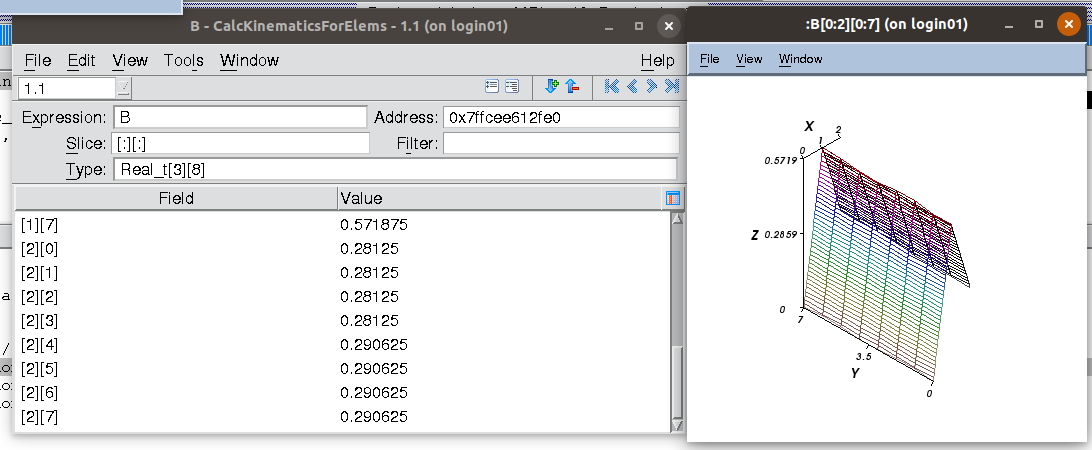
\includegraphics[width=.7\linewidth]{VisualiseArray.png}
		\caption{Visualising Array}
		\label{fig:visual_array}
		\end{center}
	\end{figure}
	
	\item \hl{What is the name of the MPI rank variable in the benchmark?}
	
	The variable is \verb!myRank!
	\item \hl{What is the name of the MPI size variable in the benchmark?}
	
	The variable is \verb!numRanks!
	\item \hl{Where are these variables first set in the benchmark’s source code (file name and line number)?}
	
	When analysing the MPI function, we run on one node with 27 processes due to limited availability of nodes.
	We set breakpoints on lines 2708 and 2709. At breakpoint 2708, prior to the execution of \verb!MPI_Comm_size()!, we see that the variables \verb!numRanks! and \verb!myRank! are uninitialized and still contain trash values in Fig. \ref{fig:before_init}. 
	After \verb!MPI_Comm_size()! runs, we see that the values across the multiple processes all show 27 in Fig. \ref{fig:init_numranks}, which is the total number of threads. 
	The value of \verb!myRank! is still unchanged and is yet to be initialized. This then occurs when we look at the values of \verb!myRank! after \verb!MPI_Comm_rank()! is run, as seen in Fig. \ref{fig:init_myrank}. 
	\verb!numRanks! is set by \verb!MPI_Comm_size()! in lulesh.cc in line 2708 and \verb!myRank! is set by \verb!MPI_Comm_rank()! in lulesh.cc line 2709. 
	
	\begin{figure}[p] % h=here, t=top, b=bottom, p=(extra)page, !=force
		\begin{center}
			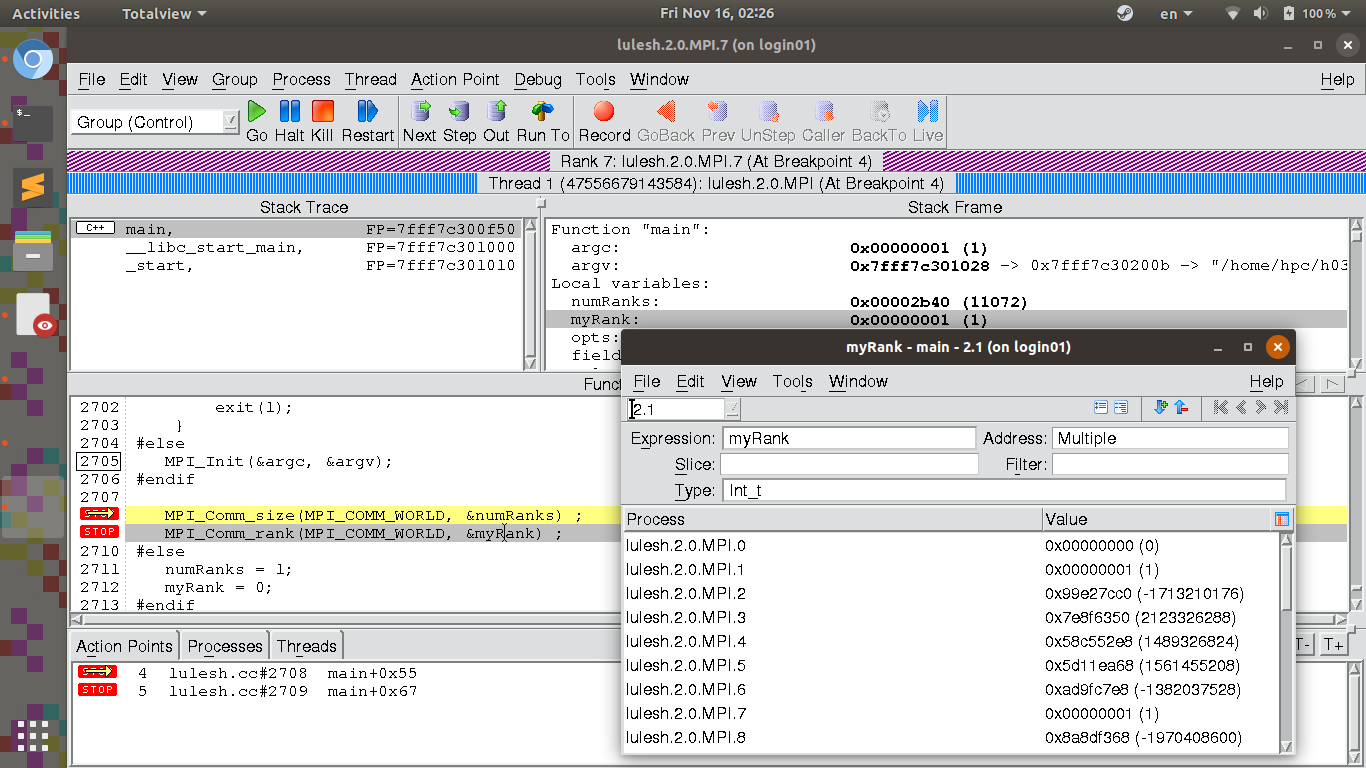
\includegraphics[width=.7\linewidth]{StepBeforeInit.png}
		\caption{Before Initialising myRank and numRanks}
		\label{fig:before_init}
		\end{center}
	\end{figure}
	
	\begin{figure}[p] % h=here, t=top, b=bottom, p=(extra)page, !=force
		\begin{center}
			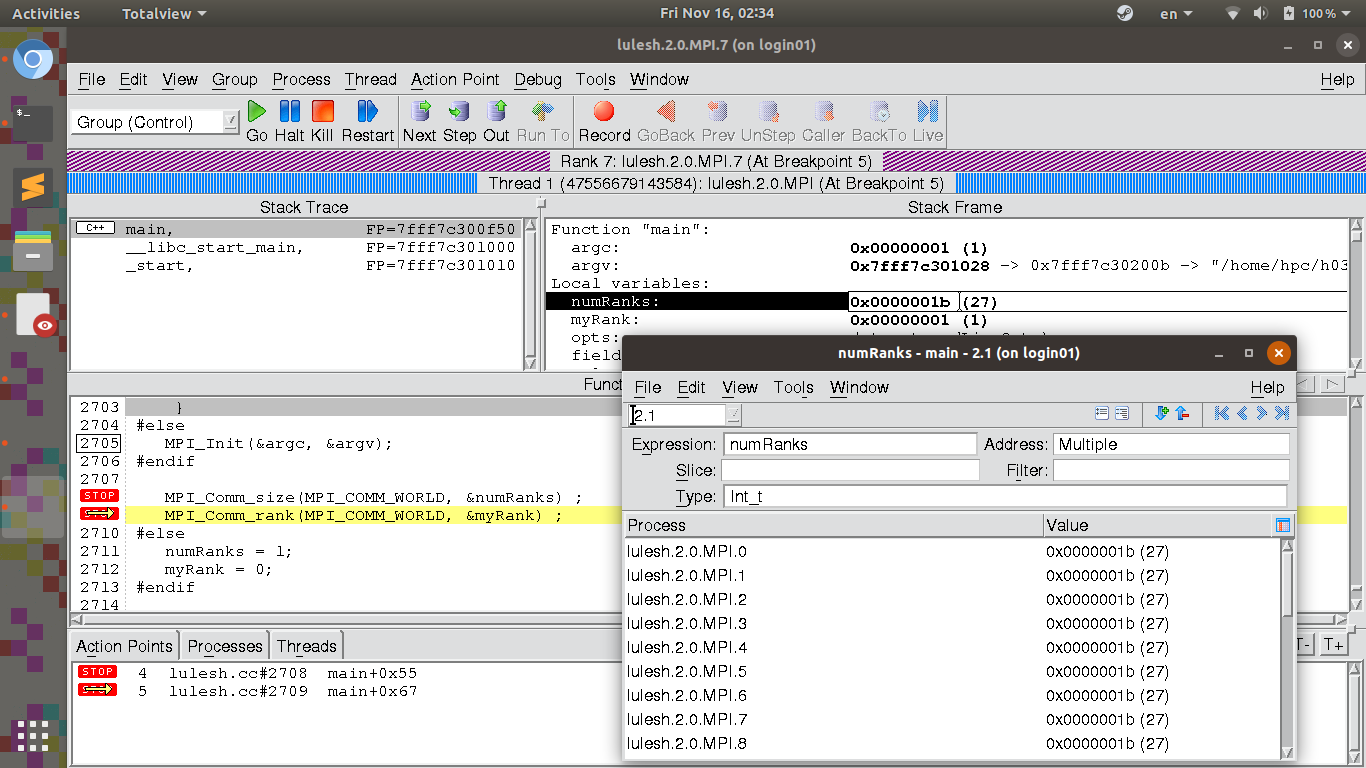
\includegraphics[width=.7\linewidth]{numRankInit.png}
		\caption{Initialised numRanks}
		\label{fig:init_numranks}
		\end{center}
	\end{figure}
	
	\begin{figure}[p] % h=here, t=top, b=bottom, p=(extra)page, !=force
		\begin{center}
			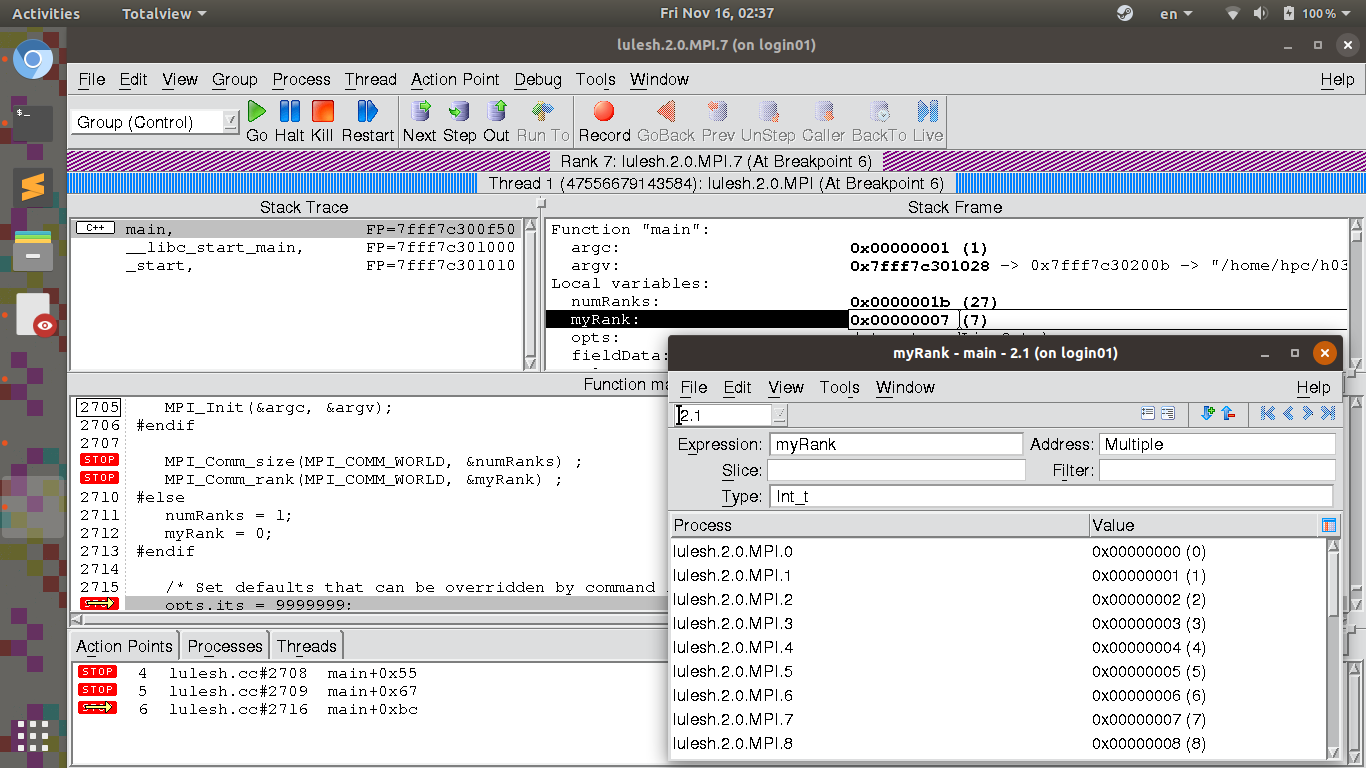
\includegraphics[width=.7\linewidth]{myRankInit.png}
		\caption{Initialised myRank}
		\label{fig:init_myrank}
		\end{center}
	\end{figure}

\end{enumerate}

\section{Task 6: MPI+OpenMP with Vampir}
\begin{enumerate}
	\item \hl{What are the main differences in the way events are recorded by gprof and Score-P?} ~

	Profiling v.s. tracing.\todo{Complete this}

	\item \hl{Does Vampir support post-mortem or online analysis? Explain.} ~

	Post-mortem?\todo{Check}

	\item \hl{Explain the communication bottlenecks that occur in point-to-point and collective MPI communication. For example, late-sender, ...} ~

	www

	\item \hl{Take a screen capture of one of the MPI communication bottlenecks from the above question, and describe the situation.} ~

	\item \hl{How does the Performance Radar help in analysis?} ~

	\item \hl{Describe the MPI message pattern in the Communication Matrix tab.} ~

	\item \hl{Take a screen capture of a fork-join, and describe the situation.} ~

	\item \hl{Do you observe any performance bottlenecks from Section 3.1 (Task 1) in the code?} ~
\end{enumerate}

\listoftodos[TODO List (to be removed in final version)]

\end{document}

%eof
